\documentclass{scrartcl}
\usepackage[a4paper,left=1in,right=1in,top=1.2in,bottom=1in]{geometry}
\usepackage{siunitx}
\usepackage{graphicx}
\usepackage{mathtools}
\setkomafont{disposition}{\normalfont\bfseries}
\newcommand*\diff{\mathop{}\!\mathrm{d}}
\newcommand*\Diff[1]{\mathop{}\!\mathrm{d^#1}}
\newcommand*\colvec[3][]{
    \begin{pmatrix}\ifx\relax#1\relax\else#1\\\fi#2\\#3\end{pmatrix}
}

%title
\title{Exercise 03:\\Development of ocular dominance}
\subtitle{Theoretical Neuroscience II}
\author{Johannes G\"atjen \and Lorena Morton}

%use these for structure/overview
\newcommand\Question{%
  \textbf{Question:}%
}
\newcommand\Answer{%
  \textbf{Answer:}%
}

\begin{document}
\maketitle

\section{Input covariance}

We choose three different values for $\gamma$ ($\gamma_1=0.5, \gamma_2=1, \gamma_3=1.5$) and compute the covariance matrices $\mathbf{C}$. The $c_S$ value does not change with $\gamma$ and is computed as 
\begin{align*}
c_S &= \langle u_Ru_R \rangle - \langle u_R \rangle^2 \\
&= \left(1 \cdot 1 \cdot \frac{1}{2} + 0 \cdot 0 \cdot \frac{1}{2}\right) - \left(1 \cdot \frac{1}{2} + 0 \cdot \frac{1}{2}\right)^2 \\
&= \frac{1}{2} - \frac{1}{4} = \frac{1}{4}
\end{align*}
The values for $c_D$ are
\begin{align*}
c_D =& \langle u_Ru_L \rangle - \langle u_R \rangle \langle u_L \rangle \\
\gamma_1: \qquad =& 1 \cdot 1 \cdot \frac{1}{8} - \frac{1}{2} \cdot \frac{1}{2} = - \frac{1}{8} \\
\gamma_2:\qquad =& 1 \cdot 1 \cdot \frac{1}{4} - \frac{1}{2} \cdot \frac{1}{2} = 0 \\
\gamma_3:\qquad =& 1 \cdot 1 \cdot \frac{3}{8} - \frac{1}{2} \cdot \frac{1}{2} = \frac{1}{8}.
\end{align*}
With a large enough sample size the numerical estimate of the covariances corresponds well with the analytical result.

\begin{figure}
\centering
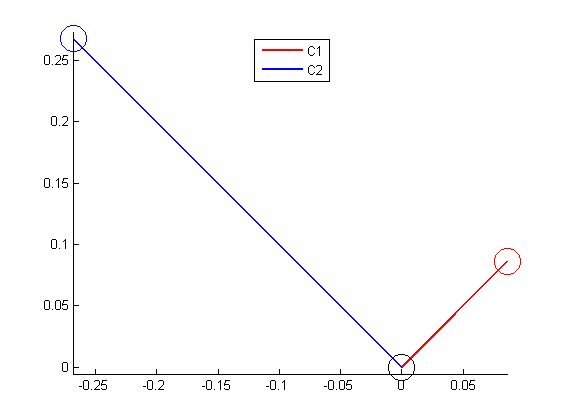
\includegraphics[trim = {1.0cm 0 0.5cm 0.2cm}, width=0.3\textwidth, clip]{../pics/g1v}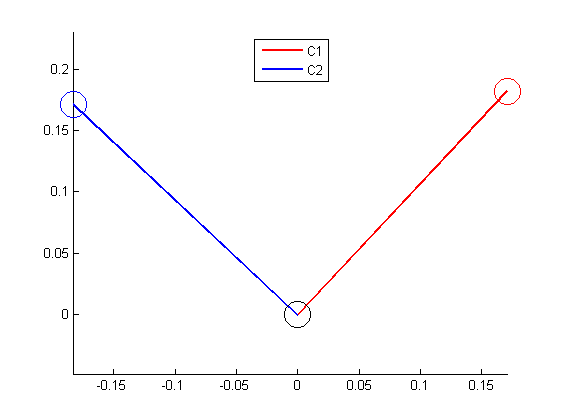
\includegraphics[trim = {1.0cm 0 0.5cm 0.2cm}, width=0.3\textwidth, clip]{../pics/g2v}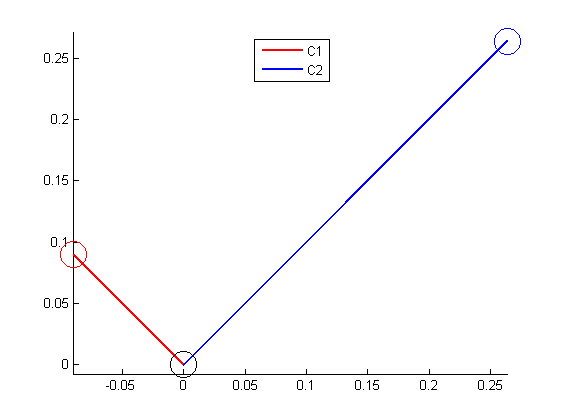
\includegraphics[trim = {1.0cm 0 0.5cm 0.2cm}, width=0.3\textwidth, clip]{../pics/g3v}
\caption{Left to right: The eigenvectors of the covariance matrices for $\gamma_1, \gamma_2$ and $\gamma_3$ respectively. With the negative correlation the $[-1, 1]$ eigenvector dominates. With no correlation the two eigenvectors are equally long. With the positive correlation the $[1, 1]$ eigenvector dominates.}
\end{figure}

\section{Development with weight saturation}

Next we develop the input weights $\mathbf{w} = [w_L, w_R]^T$ for a neuron according to the covariance rule
\begin{align*}
\tau \frac{\diff \mathbf{w}}{\diff t} = \mathbf{C} \mathbf{w} \\
\shortintertext{which evaluates to}
\tau \colvec{\frac{\diff w_L}{\diff t}}{\frac{\diff w_R}{\diff t}} = \colvec{w_Lc_S + w_Rc_D}{w_Lc_D + w_Rc_S}
\end{align*}
giving us effectively two differential equations to use for update rules.

Figure \ref{cov} shows the development of the weights for the different values for $\gamma$ and random starting positions. With $\gamma = 1$ the weights develop entirely proportional to the initial condition, until they get to the boundary condition and eventually converge in the state for binocular vision. For $\gamma = 1.5$ the weights always grow roughly in the direction of the principal eigenvector, also converging in the state for binocular vision. With $\gamma = 0.5$ the weights also tend to grow in the direction of the principal eigenvector, but because of the weight saturation rule, whether the final state is monocular or binocular depends on the initial conditions of the weights. Where the initial weights are dissimilar and small enough the weights converge to monocular vision for the side with the higher initial weight. On the other hand, when the initial weights are too large or very similar the system will end in the binocular state.

In conclusion, for monocular neurons to develop, it is necessary, that the inputs are anti-correlated and the initial connection weights are not too similar.

\begin{figure}
\centering
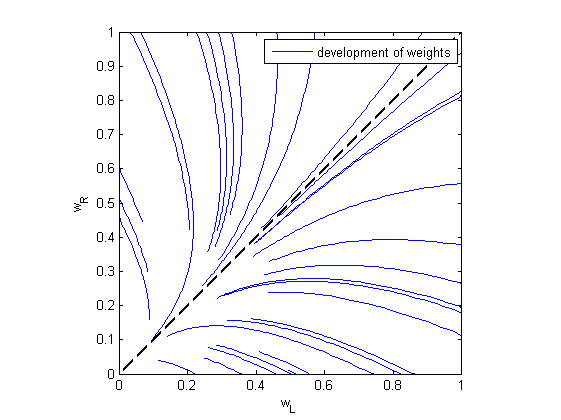
\includegraphics[trim = {1.8cm 0 2.5cm 0.4cm}, width=0.4\textwidth, clip]{../pics/g1t1}
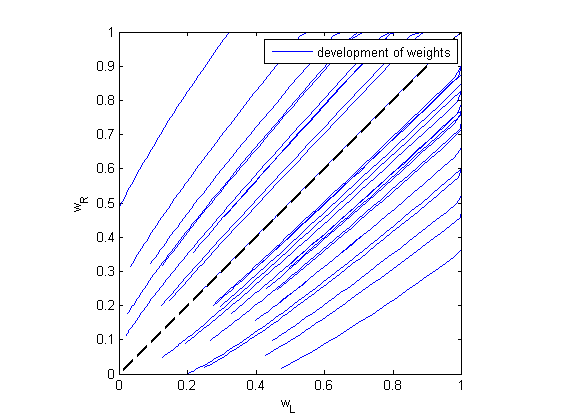
\includegraphics[trim = {1.8cm 0 2.5cm 0.4cm}, width=0.4\textwidth, clip]{../pics/g3t1}
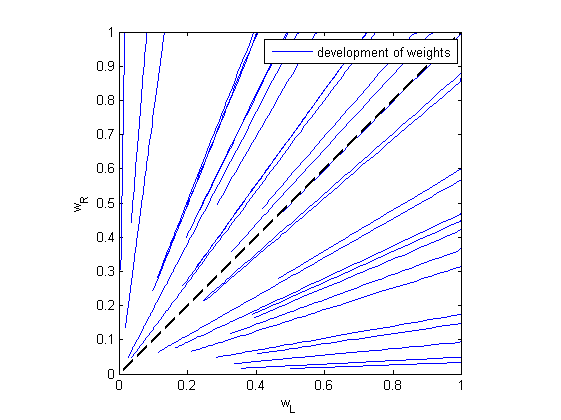
\includegraphics[trim = {1.8cm 0 2.5cm 0.4cm}, width=0.4\textwidth, clip]{../pics/g2t1}
\caption{Development of connection weights with the covariance rule for different starting values in the range of $[0..0.5]$ and three different values for $\gamma$ ($\gamma = 0.5$ top left, $\gamma = 1.5$ top right, $\gamma = 1$ bottom).}
\label{cov}
\end{figure}

\section{Development with dynamic normalization}

Now we modify our update rule to include a dynamic normalization:
\begin{align*}
\tau \frac{\diff \mathbf{w}}{\diff t} &= \mathbf{C} \mathbf{w} - \frac{1}{2} \left( \mathbf{w}^T \mathbf{C} \mathbf{w} \right) \mathbf{w} \\
\text{Let } N &= \mathbf{w}^T \mathbf{C} \mathbf{w} \\
&= \colvec{w_L}{w_R}^T \colvec{w_Lc_S + w_Rc_D}{w_Lc_D + w_Rc_S} \\
&= w_L(w_Lc_S + w_Rc_D) + w_R(w_Lc_D + w_Rc_S) \\
&= w_L^2c_S + 2 w_Rw_Lc_D + w_R^2c_S
\shortintertext{and the update rule evaluates to}
\tau \colvec{\frac{\diff w_L}{\diff t}}{\frac{\diff w_R}{\diff t}} &= \colvec{w_Lc_S + w_Rc_D}{w_Lc_D + w_Rc_S} - \frac{N}{2} \colvec{w_L}{w_R}
\end{align*}

Figure \ref{dyn} shows the same initial conditions and $\gamma$ values as Figure \ref{cov} with the dynamic normalization rule added. In the case of $\gamma = 1$ there is no apparent difference to the development without the dynamic normalization. With $\gamma = 1.5$ the convergence towards the binocular state is stronger than without the dynamic normalization, making no difference for the final state. In the case of the anti-correlated input however, the weights now always end in the state for the monocular neuron where the side with the larger initial value is preferred. This means, that for this model it is sufficient that the inputs are anti-correlated and the initial weights are not exactly equal for monocular neurons to develop.

\begin{figure}
\centering
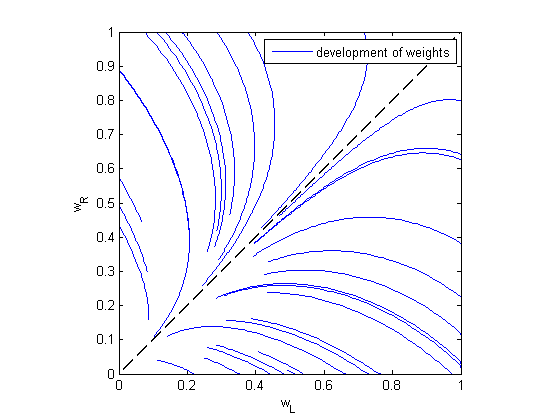
\includegraphics[trim = {1.8cm 0 2.5cm 0.4cm}, width=0.4\textwidth, clip]{../pics/g1t2}
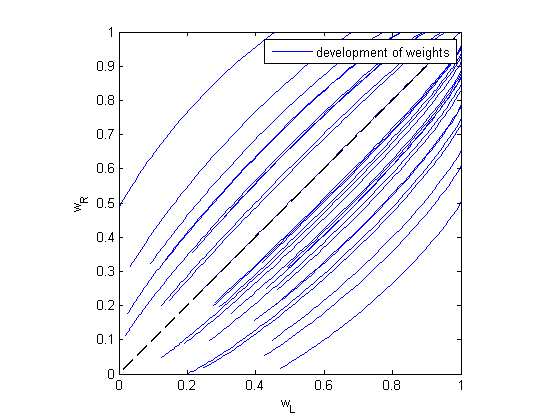
\includegraphics[trim = {1.8cm 0 2.5cm 0.4cm}, width=0.4\textwidth, clip]{../pics/g3t2}
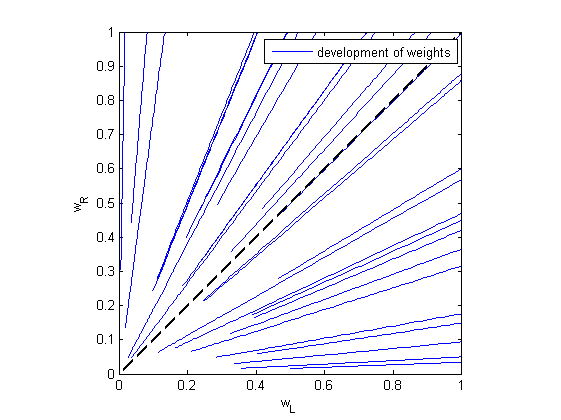
\includegraphics[trim = {1.8cm 0 2.5cm 0.4cm}, width=0.4\textwidth, clip]{../pics/g2t2}
\caption{Development of connection weights with the covariance rule for different starting values in the range of $[0..0.5]$ and three different values for $\gamma$ ($\gamma = 0.5$ top left, $\gamma = 1.5$ top right, $\gamma = 1$ bottom), including dynamic normalization.}
\label{dyn}
\end{figure}

\end{document}